\chapter*{Введение}

В настоящее время как в нашей стране, так и за рубежом всё большее внимание уделяется созданию различных типов беспилотных летательных аппаратов. 


Использование беспилотного летательного аппарата может обеспечить преимущество по сравнению с пилотируемыми. Это связано с тем обстоятельством, что беспилотные летательные аппараты имеют ряд преимуществ перед пилотируемыми, в частности для них:
\begin{itemize}
\item устанавливаются существенно менее жесткие требования по безопасности конструкции
\item не требуется систем поддержания работоспособности и жизнеобеспечения экипажа
\item устанавливаются существенно менее жесткие ограничения режимов полета.
\end{itemize} 

%При их создании особое внимание уделяется требованиям малозаметности и увеличения аэродинамического качества, и как следствие, возможности барражировать в течение длительного времени. 


Благодаря этому БПЛА имеют большой потенциал для разработки для них легких и дешевых конструкций планера, что позволяет решать многие технические задачи, недоступные для пилотируемых летательных аппаратов.

В настоящее время существуют БПЛА, предназначенные для выполнения ряда задач, таких как: разведка, боевые задачи, исследования и др. На Рис.\ref{fig:UAVs} представлены некоторые из существующих БПЛА с указанием их предназначения.  

%\begin{figure}
%	\begin{subfigure}[b]{0.48\textwidth]
%		\includegraphics{UAV_Reaper}
%		\caption{MQ-9 Reaper во время боевого вылета в Афганистане, 2008 год.}
%		http://ru.wikipedia.org/wiki/MQ-9_Reaper
%		U.S. Air Force Photo / Lt. Col. Leslie Pratt - USAF Photographic Archives http://www.afrc.af.mil/shared/media/photodb/photos/090127-F-7383P-002.JPG
%	\end{subfigure}
%	~
%	\begin{subfigure}[b]{0.48\textwidth]
%		\includegraphics[width=0.4\textwidth]{UAV_X47}
%		\caption{X-47A на выкате}
%		%http://ru.wikipedia.org/wiki/X-47_Pegasus
%		%http://archive.darpa.mil/j-ucas/X-47/gallery/X-47A/hi_res/pegasus2_hi-res.jpg
%	\end{subfigure}
%	\caption{Shit}
%	\label{UAVs}
%\end{figure}

\begin{figure}[H]
        \begin{subfigure}[b]{0.47\textwidth}
                \includegraphics[width=\linewidth]{UAV_Reaper}
                \caption{MQ-9 Reaper, разведывательно-ударный} % http://ru.wikipedia.org/wiki/MQ-9_Reaper , U.S. Air Force Photo / Lt. Col. Leslie Pratt - USAF Photographic Archives http://www.afrc.af.mil/shared/media/photodb/photos/090127-F-7383P-002.JPG
                \label{fig:UAV_Reaper}
        \end{subfigure}%
        \hspace{\fill}
        \begin{subfigure}[b]{0.47\textwidth}
                \includegraphics[width=\linewidth]{UAV_X47}
                \caption{Northrop X-47A, боевой} %http://ru.wikipedia.org/wiki/X-47_Pegasus
%		%http://archive.darpa.mil/j-ucas/X-47/gallery/X-47A/hi_res/pegasus2_hi-res.jpg
                \label{fig:UAV_X47}
        \end{subfigure}%
        \hspace{\fill}\linebreak
        \begin{subfigure}[b]{0.47\textwidth}
                \includegraphics[width=\linewidth]{UAV_X45}
                \caption{Boeing X-45C, экспериментальный многоцелевой}
%http://ru.wikipedia.org/wiki/Boeing_X-45
                \label{fig:UAV_X45}
        \end{subfigure}%
        \hspace{\fill}
        \begin{subfigure}[b]{0.47\textwidth}
                \includegraphics[width=\linewidth]{UAV_RQ7}
                \caption{RQ-7A Shadow 200, разведывательный}
                \label{fig:UAV_RQ7}
        \end{subfigure}
        \caption{Некоторые существующие БПЛА}\label{fig:UAVs}
\end{figure}






%Рассказать про беспилотник (типы, картинки), предназначены для решения ряда задач.

%Дальше про разные типы.

Одной из основных задач беспилотных самолетов является военный и гражданский мониторинг. Такие самолеты предназначены для продолжительного ($\approx24$ часа для !привести пример!) скрытного барражирования без дозаправки, что накладывает высокие требования по малозаметности, высокой весовой эффективности и высокому аэродинамическому качеству.

%Основное - мониторинг (военный, гражданский). Из этого следуют требования малозаметности и весовой эффективности.

%Использование беспилотника может обеспечить преимущество по сравнению с пилотируемыми, почему.

%Показать несколько существующих и разрабатываемых БПЛА для мониторинга.

Для обеспечения малозаметности БПЛА при проектировании самолета самолет создают наиболее ``плоским'' -- конструкция создается с минимально возможной строительной высотой. Для достижения высокого аэродинамического качества используют крылья большого удлинения и принципиальную схему ``летающее крыло''. Использование крыльев большого удлинения влечет за собой появление больших изгибающих моментов в центроплане, и для обеспечения прочности конструкции используют интегральный центроплан. 

%Объясняем, почему нужна интегральная схема и крыло большого удлинения. Цель - меньше заметности следовательно уменьшение строительной высоты, больше аэродинамического качество.

Кроме того, из необходимости уменьшения строительной высоты возникает проблема интеграции двигателя и центроплана. Одним из решений данной проблемы является использование центроплана, имеющего изгиб в фюзеляжной части. (Рис.\ref{fig:OriginalSectionWithEngine}). 

%Выходим на основную проблему. Проблема интеграции двигателя и центроплана. Описанные выше требования приводят к проблемам. 

%Показываем наш БПЛА (модель из катьи), одним из решений является изогнутый центроплан.

\begin{figure}[ht]
\captionsetup{justification=centering}
\centering
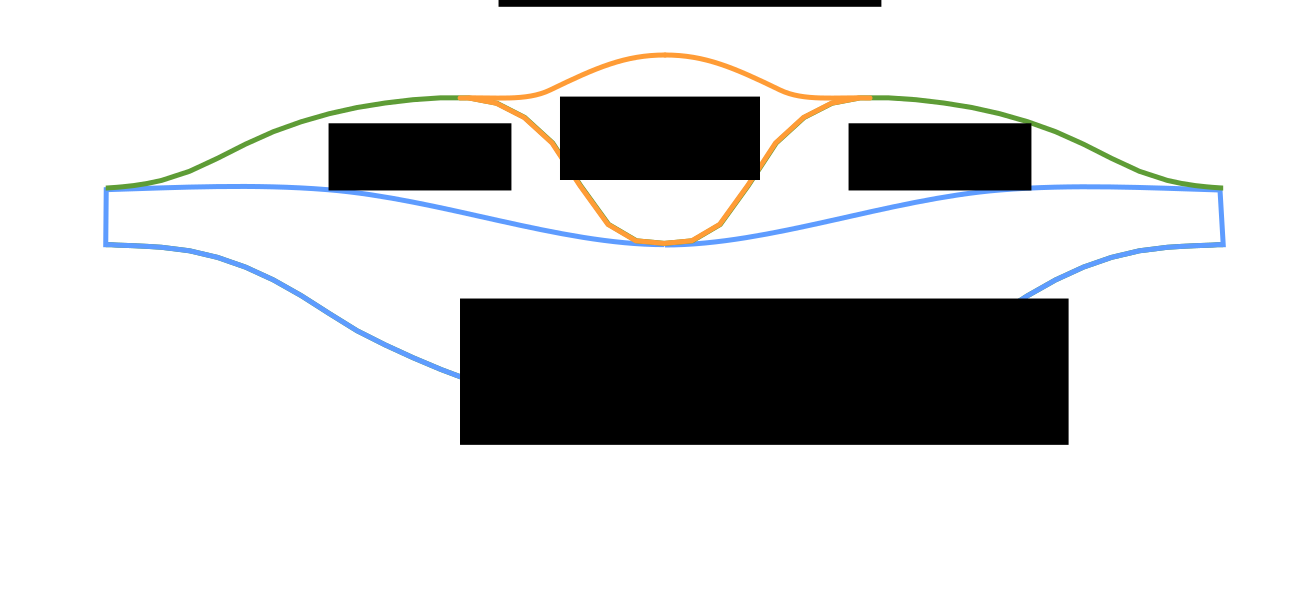
\includegraphics[width=0.8\textwidth]{OriginalSectionWithEngine}
\caption{Вид сечения центроплана в месте стыка передней кромки крыла и фюзеляжа с изображением двигателя}
\label{fig:OriginalSectionWithEngine}
\end{figure}


При использовании такого решения требования малозаметности и высокого аэродинамического качества могут быть выполнены, но наличие изгиба приводит к проблеме обеспечения прочности центроплана и, как следствие, обеспечения весовой эффективности самолета. 
%При такой конфигурации все хорошо (учтены требования малозаметности, аэродинамики).

В настоящей работе рассматривается задача проектирования конструкции центроплана беспилотного летательного аппарата с интеграцией двигателя и центроплана, с крылом большого удлинения, выполненного по схеме ``летающее крыло'' (Рис.\ref{fig:BPS}). Основной задачей при проектировании является обеспечение достаточной прочности при заданных аэродинамических и массовых нагрузках.


\begin{figure}[ht]
\centering
\includegraphics[width=0.8\textwidth]{BPS_Catia}
\caption{Проектируемый БПЛА}
\label{fig:BPS}
\end{figure}



%Но это создает проблему обеспечения прочности центроплана, следовательно проблему весовой эффективности. Наше решение - критическое к созданию конструкции. Если не выйдет, всё летит к черту. Создаем модель по идеальной аэродинамике.

%В настоящей работе рассматривается задача проектирования такой конструкции центроплана БПЛА с особенностью, с крылом большого удлинения.


Для решения задачи в работе проведено концептуальное исследование зависимости весовых, прочностных и жесткостных характеристик конструкции от геометрических параметров, определяющих форму центроплана.

Однако, при исследовании влияния изменения формы центроплана на характеристики ЛА необходимо также учитывать изменения в аэродинамических характеристиках ЛА. 

В рамках решения задачи сформирован задел для дальнейшего решения многодисциплинарной задачи по выбору рациональной конфигурации и улучшению компоновки проектируемого самолета с точки зрения критерия эффективности с учетом возможного изменения внешней геометрии и, как следствие, возможного изменения аэродинамических характеристик самолета. 

В работе также рассмотрены программные средства, предназначенные для решения подобных (параметрических, проектировочных) задач, проведены модификации данных программных средств и приведено описание модификаций.  

В работе сформирована параметрическая МКЭ-модель, пригодная для дальнейших исследований в решении многодисциплинарной задачи, и проведены валидационные исследования этой модели. Проведены весовые оценки конструкции на основе расчета МКЭ-модели.   

 